\documentclass[../main.tex]{subfiles}
\begin{document}

\chapter{Lecture 16 - 05-05-2020}

\section{Analysis of Perceptron in the non-separable case using OGD framework.}
We are finishing up the part of online learning and gradiant descent. \\
Concrete example for the parameter G:
$$
G = \max_t \| \nabla \ell_t(w_t) \|^2 \qquad \ell_t(w) = (w^T \, x_t -y_t)^2 \qquad \|x_t\| \leq X, |y_t| \leq U\, X
$$
$$
\|w\| \leq U, |w^T \, x_t| \leq \| w \| \, \| x_t \|
$$
where $\| w \| \rightsquigarrow U$
and $\|x_t\| \rightsquigarrow X$ (so are bounded by U and X)
\\\\
Now we want to find the gradiant.
\\
$$
\| \nabla \ell_t(w) \| \leq 2 \, | w^T \, x_t - y_t | \, \|x_t \| \leq 4 \, U \, X \| x_t \| \leq 4 \, U \, X^2
$$
where $w^T \, x_t \ bounded \ U \, X$ and $y_t$ bounded by $U \, X$
$$
R_T(u) = U \, G  \ \sqrt[]{8T} \leq 8 (UX)^2 \ \sqrt[]{2 \, T}
$$
How about OGD for classification?\\
The problem is that zero-one loss is not convex (also non-continous).
\\
$$
I \{ y_t \, w^T \, x_t \leq 0 \}
$$
This is zero-one loss for linear classification.
\begin{figure}[h]
    \centering
    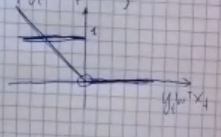
\includegraphics[width=0.4\linewidth]{../img/lez16-img1.JPG}
    \caption{}
    %\label{fig:}
\end{figure}\\
$$
w \leftarrow w - \eta \, \nabla \ell_t(w) \qquad \bred{OGD}
$$
$$
w \leftarrow w + y_t \, x_t \, I \{ y_t \, w^T \, x_t \leq 0 \} \qquad \bred{Perceptron}
$$
We want to make this equal with loss that is convex and also tell us bound with zero one loss. So there is a bunch or problem.
\\
So we want to make this equal but how? 
\\
$$
\ell_t(w) = \left[ -y_t \, w^T \, x_t \right]_+ \qquad \left[ z \right]_t = \max \{0,z\}
$$ \
If we take the gradiant of this with respect to $w$:
$$
\nabla \ell_t(w) = -y_t \, x_t \, I \{ y_t \, w^T \, x_t \leq 0 \}
$$
Now - this gradiant is exactly this $\ell_t(w) = \left[ -y_t \, w^T \, x_t \right]_+ $ 
\\
The problem is not comparable with the number of mistakes so I am not going to have the number of mistakes. 
\\\\How do I do it? 
\\
What if I just shift to the right? \\
Now this loss is an upper bound of the zero-one loss. And this is called \bred{Hinge loss} (where hinge take the door attached to the frame of the wall)\\
\begin{figure}[h]
    \centering
    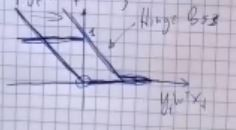
\includegraphics[width=0.4\linewidth]{../img/lez16-img2.JPG}
    \caption{Hinge loss}
    %\label{fig:}
\end{figure}\\
$$
\textbf{Hinge loss: } \ h_t(w) = \left[ 1 - y_t \, w^T \, x_t \right]_+ \geq I \{ y_t \, w^T \, x_t \leq 0 \}
$$
$$
\nabla h_t(h) = - y_t \, x_t \, I\{y_t \, w^T \, x_t \leq 1 \}
$$
The problem is that it becames 0 later on than the original one.
\\
$$
w \leftarrow w - \eta \, \nabla h_t(w) \, I \{ y_t \, w^T x_t \leq 0\}
$$
$$
y_t \, w^T \, x_t \leq 0 \ \ \Rightarrow \ \ y_t \, w^T x_t \, \leq 1
$$
We now apply OGD analysis to $h_t$ considering only the steps $T$ where $I \{ y_t \, w_t^T \, x_t \leq 0  \} 
$ and we do not perform projection. 
$$
\sum_{t=1}^T \left( h_t \left(w_t \right) - h_t(u) \right) \ I\{y_t \, w_t^T \, x_t \leq 0 \} \leq 
$$
$$ \leq \ \frac{1}{2 \, \eta} \, \| U \|^2 + 
\red{
\frac{1}{2} \, \sum_{t=1}^T \| w_{t+1} - u \| \, \left( \frac{1}{\eta} - \frac{1}{\eta} \right) \, I \{y_t \, w_t^T \, x_t \leq 0 \} 
}
+ \frac{\eta \, G^2}{2} \, \sum_{t=1}^T I \{y_t \, w_t^T x_t \leq 0 \}
$$
where second factor cancel out
$$
- \frac{1}{2 \, \eta} \| w_{T+1} - u \|^2 \qquad \| \nabla h_t(w) \| = |y_t| \| x_t \| \leq X \qquad G = X = \max_t \| x_t \|
$$
where $y_t$ in $\{ -1,1\}$
$$
y_t \, w_t^T \, x_t \leq 0 \ \Rightarrow \ h_t(w_t) \geq 1
$$
\\
\begin{figure}[h]
    \centering
    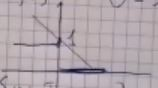
\includegraphics[width=0.4\linewidth]{../img/lez16-img3.JPG}
    \caption{}
    %\label{fig:}
\end{figure}\\
$$
\sum_{t=1}^T I \{y_t \, w_t^T x_t \leq 0  \} \ \leq \ \sum_{t=1}^T h_t(w_t) I \{y_t \, w_t^T \, x_t \leq 0 \} \ \leq 
$$
$$
\ \sum_{t=1}^T h_t(u ) \, \red{I \{ y_t \, w_t^T \, x_t \leq 0 \}} + \frac{1}{2 \, \eta} \| u \|^2 + \frac{\eta}{2} x^2 \, \sum_{t=1}^T I\{y_t w_t^T \, x_t \leq 0 \}
$$
where $I{..}$ cancel out to have a "nicer" upper bound.
$$
M_T = \sum_{t=1}^T  I\{y_t w_t^T \, x_t \leq 0 \}
$$
$$
M_T \leq \sum_{t=1}^T h_t(u) + \frac{1}{2 \, \eta} \|u \|^2 + \frac{\eta}{2} x^2 \ M_T
$$
This is not a regret anymore! Here \textbf{$M_T$ is the number of mistakes} and I compare it with the hinge loss ($h_t(u)$).
\\
I CAN'T USE THIS $\eta = \frac{\|u\|}{x \, \sqrt[]{M_T}}$
but we can replace it in $M_T$.
\\
$$
M_T \ \leq \ \sum_{t=1}^T h_t(u) + \|u\| X \, \sqrt[]{M_T}
$$
$$
M_T \ \leq \ \sum_{t=1}^T h_t(u) + (\| u\| x)^2 + \| u\| \, x \ \sqrt[]{\sum_t h_t(u)}
$$
$$
w \leftarrow w + \eta \, y_t \, x_t \, I\{y_t w_t^T \, x_t \leq 0 \} \qquad w = (0,...0)
$$
If I choose $\eta$ > 0?
$$
w_t = \eta \, \sum_{s=1}^{t-1} y_s \, x_s \, I\{y_s w_s^T \, x_s \leq 0 \} \qquad \forall \ \eta > 0
$$
Also holds because it's true $ \forall \eta > 0$
$$
M_T = \sum_{t=1}^T I\{y_t w_t^T \, x_t \leq 0 \} \quad \textbf{ invariant with respect to $\eta >0$}
$$
It does not matter which $\eta$ we choose. The number of mistakes is going to be the same. This mean that the state of the algorithm (which depends on mistakes) is gonna be the same.
\\
I can run perceptron with $\eta = 1$ and pretend (in the analysis) it was run with $\eta = \frac{\| U \|}{X \, \sqrt[]{M_T}}$
\\\\
We go back to the bound of $M_T$ . We are actually free to choose any number of U.
\\
If $(x_1, y_1),(x_2,y_2) $ is linearly separable then: \\ $\exists U$ s.t. $y_t \, U^T x_t \geq 1 \ \Rightarrow \ h_t(u) = 0 \ \ \forall t $
\\
$$M_T \ \leq \ \left( \, \| U\| \ X \, \right)^2  \qquad the \ \bred{perceptron convergence theorem.} $$
$$
M_T \ \leq \ \min_{u \in \barra{R}^d} \left( \sum_{t=1}^T h_t(u) + \left( \|U\| \, X \right)^2 + \| U \| \, X \ \sqrt[]{\sum_t h_t(u)} \right)
$$
This are called \bred{Oracle bounds}, the perceptron knows which is the best $U$.
\newpage
\subsection{Strongly convex loss functions}
We use this to analyse all class of algorithms that regularise the ERM which is the support vector machine. We want to explain what happen using Support vector Machine. For neural networks we cannot do this since NN are not convex and there is not way to "convexify". Convexifying we lose the power of NN.
\\
We said that $\ell_t$ have to be convex. But i have a lot of types of convexity.
\\
\begin{figure}[h]
    \centering
    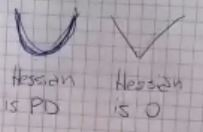
\includegraphics[width=0.4\linewidth]{../img/lez16-img4.JPG}
    \caption{Example of more type of convex function}
    %\label{fig:}
\end{figure}\\
This two for example are both convex. In the left this always has a positive curvature, while the right one we have a 0 curvature since is two straight line and not differentiable.
In other word, Hessian on the left positive and definite. On the right Hessian is 0.
\\
We are looking for \bred{strongly convex losses}.
\\
$\ell$ differentiable is $\sigma$-$strongly$ convex if:
$$
\forall u,w \qquad \ell(w) - \ell(u) \leq \nabla \ell(w)^T \, (w-u) - \frac{\sigma}{2}
 \, \| w-u\|^2 \qquad \sigma > 0$$
$\sigma$-$SC$ is equivalent to the Hessian having all strictly positive eigeinvalues.
\\\\\\
Example, check if strictly convex:
\\
$$
\ell(w) = \frac{1}{2} \| w\|^2 \qquad \frac{1}{2} \| w\|^2 - \frac{1}{2} \| u\|^2   \ \leq^? \ w^T \, (w-u) - \sigma \, \frac{\| w-u\|^2}{2} 
$$
whehre $\sigma = 1$
$$
\red{\frac{1}{2} \| w \|^2 }- \frac{1}{2} \|u\|^2 \ \leq^? \ \|w\|^2 - w^T \, u - \frac{\| w-u\|^2}{2}  $$
where $\frac{1}{2} \| w \|^2 $ cancel out
$$
0 \ \leq \ \frac{1}{2} \| w\|^2 + \frac{1}{2} \|u\|^2 - \frac{\| w-u\|^2}{2} - w^T \, u
$$
I put $ 0 = ... $
$$
0 \ = \ \frac{1}{2} \| w\|^2 + \frac{1}{2} \|u\|^2 - \frac{\| w-u\|^2}{2} - w^T \, u
$$
So this function is $1$-\textit{strongly convex}
\\\\
Next lecture we are going to show that we can run OGD with strongly convex functions. We are going to get a better bound. Our regret is gonna vanish much faster than the case of simple convexity. 
\\
You can prove that if Hessian is 0, your regret is vanishing with a rate of $ \frac{U \, G}{\sqrt[]{T}}$.
\\
We will shows with strong convexity the OGD will converge much faster with a rate of $ \frac{ \ln T}{T}$.\\
This is what happen in optimisation, we prefer strictly convex function.
\end{document}